\documentclass[9pt]{beamer}

\usepackage{tikz}
\usepackage{amsmath}
\usepackage{physics}

\usepackage{graphicx}
\graphicspath{ {./images/}}
\setbeamertemplate{navigation symbols}{}

\usetheme{default}
\usecolortheme{beetle}
\usefonttheme{serif}

\setbeamercolor{frametitle}{fg=white}
\setbeamercolor{background canvas}{bg=black}
\setbeamercolor{normal text}{fg=white}

\newcommand{\arr}{\ensuremath{\longrightarrow}}

\title{The Statistics of Gravitational Microlensing Photometry}
\author{Jack Symonds}
\date{}

\begin{document}

\begin{frame}
\maketitle
\begin{figure}[h]
\centering
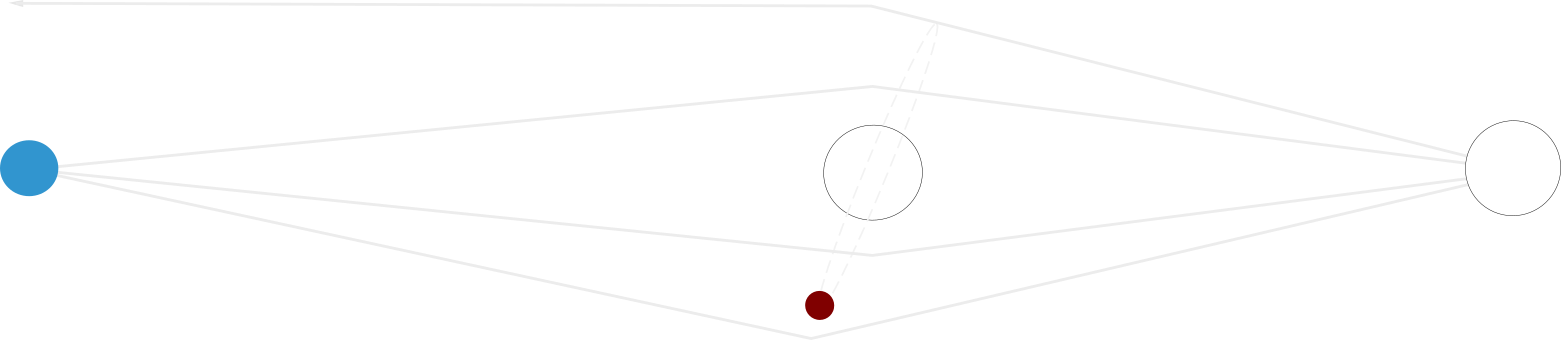
\includegraphics[width=10cm]{intro}
\end{figure}
\end{frame}

\begin{frame}
\begin{figure}[h]
\centering
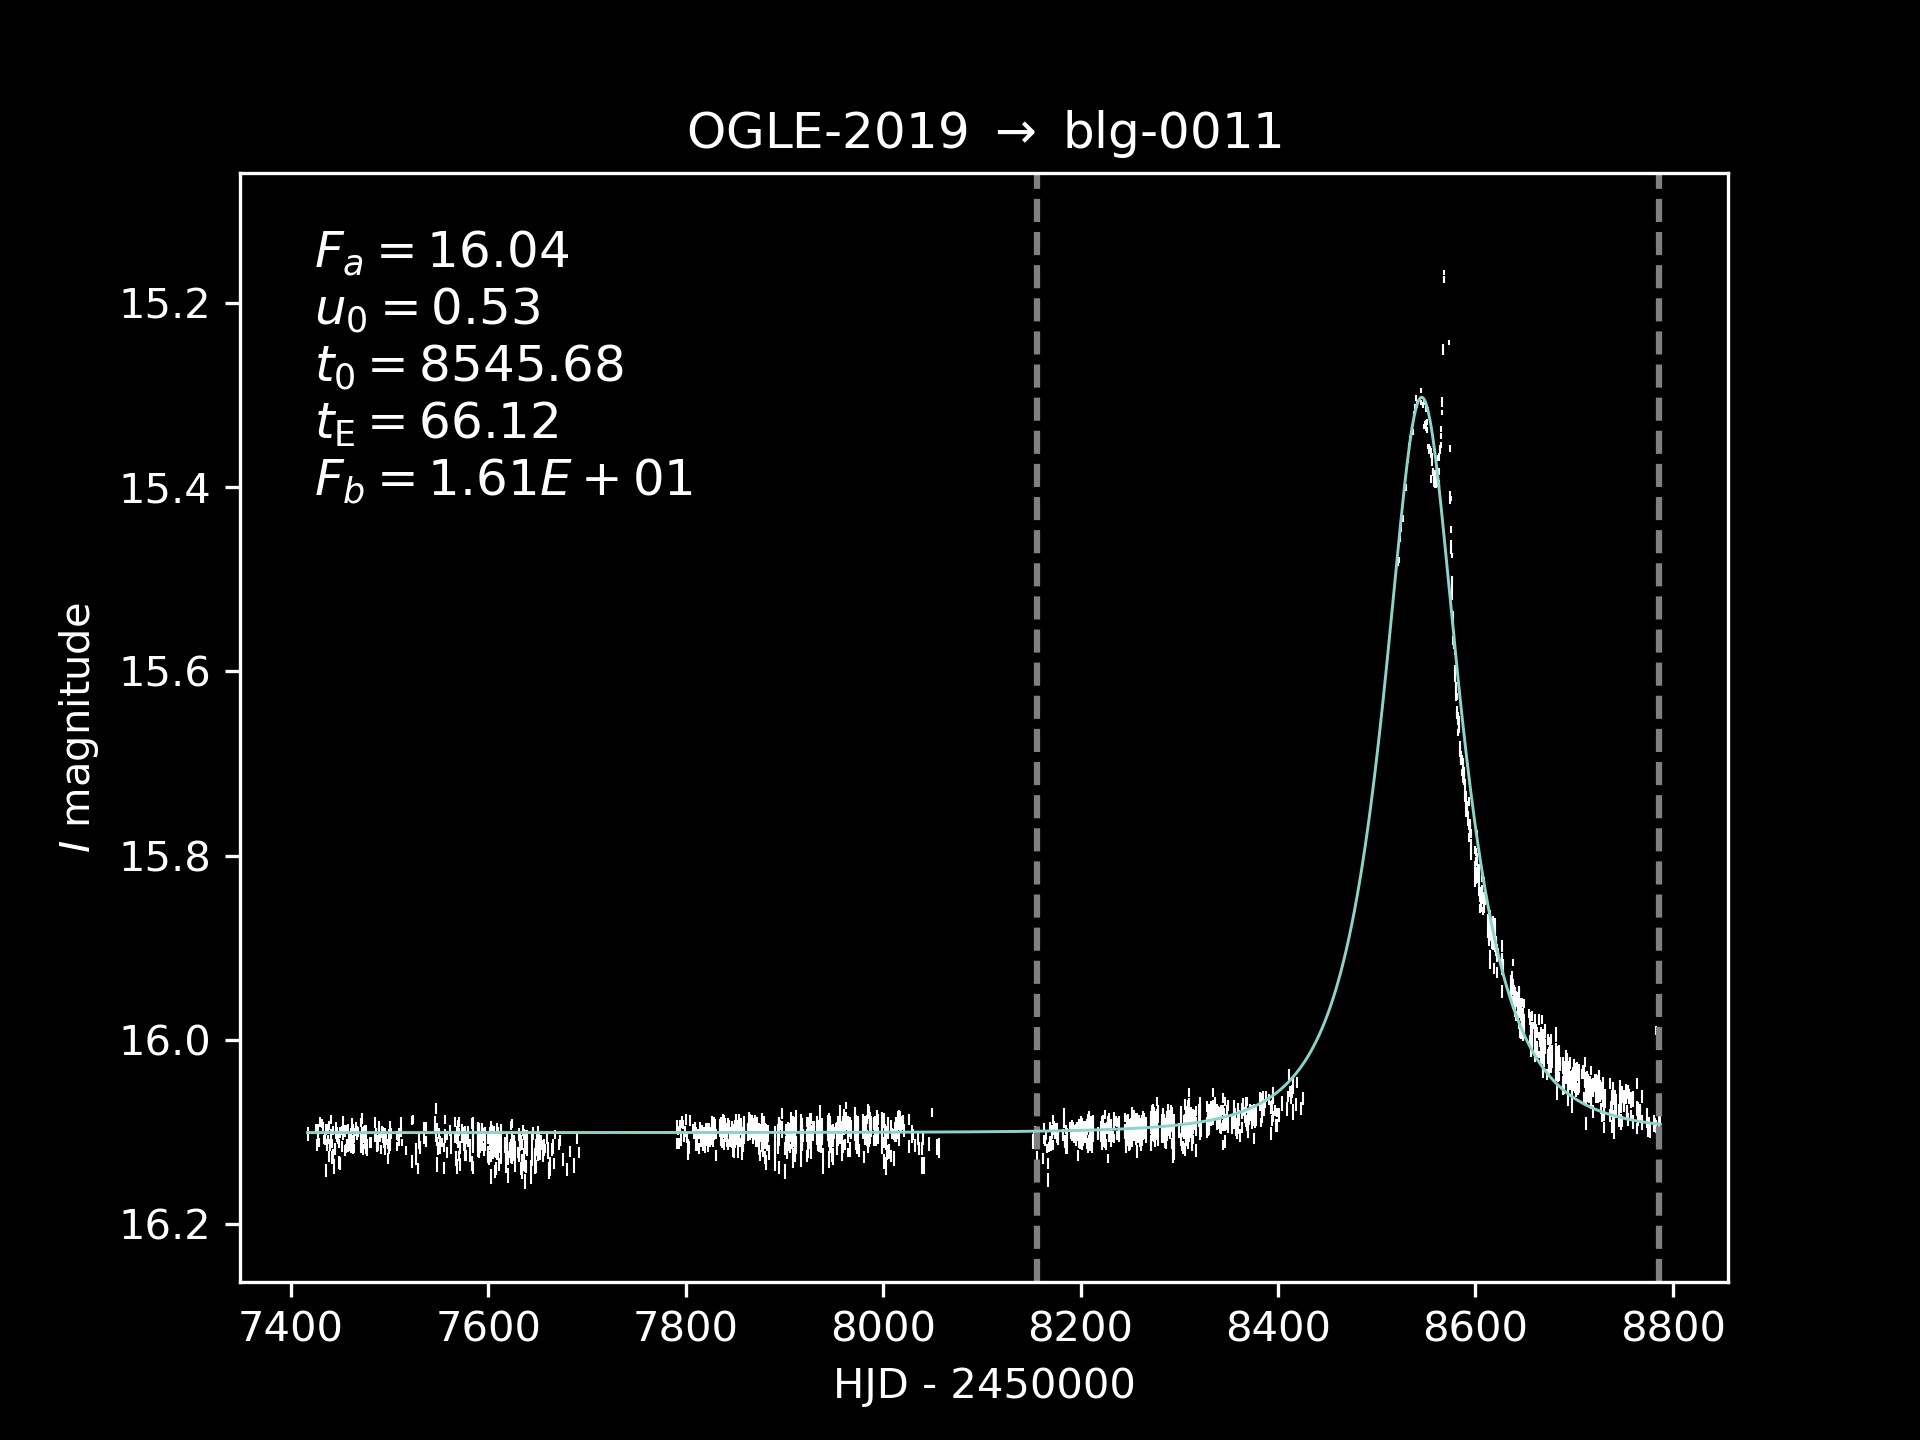
\includegraphics[width=\textwidth]{phot_dat}
\label{fig:phot_dat}
\end{figure}
\end{frame}


\begin{frame}
\frametitle{Constant Magnitude Distribution}
\begin{figure}[h]
\centering
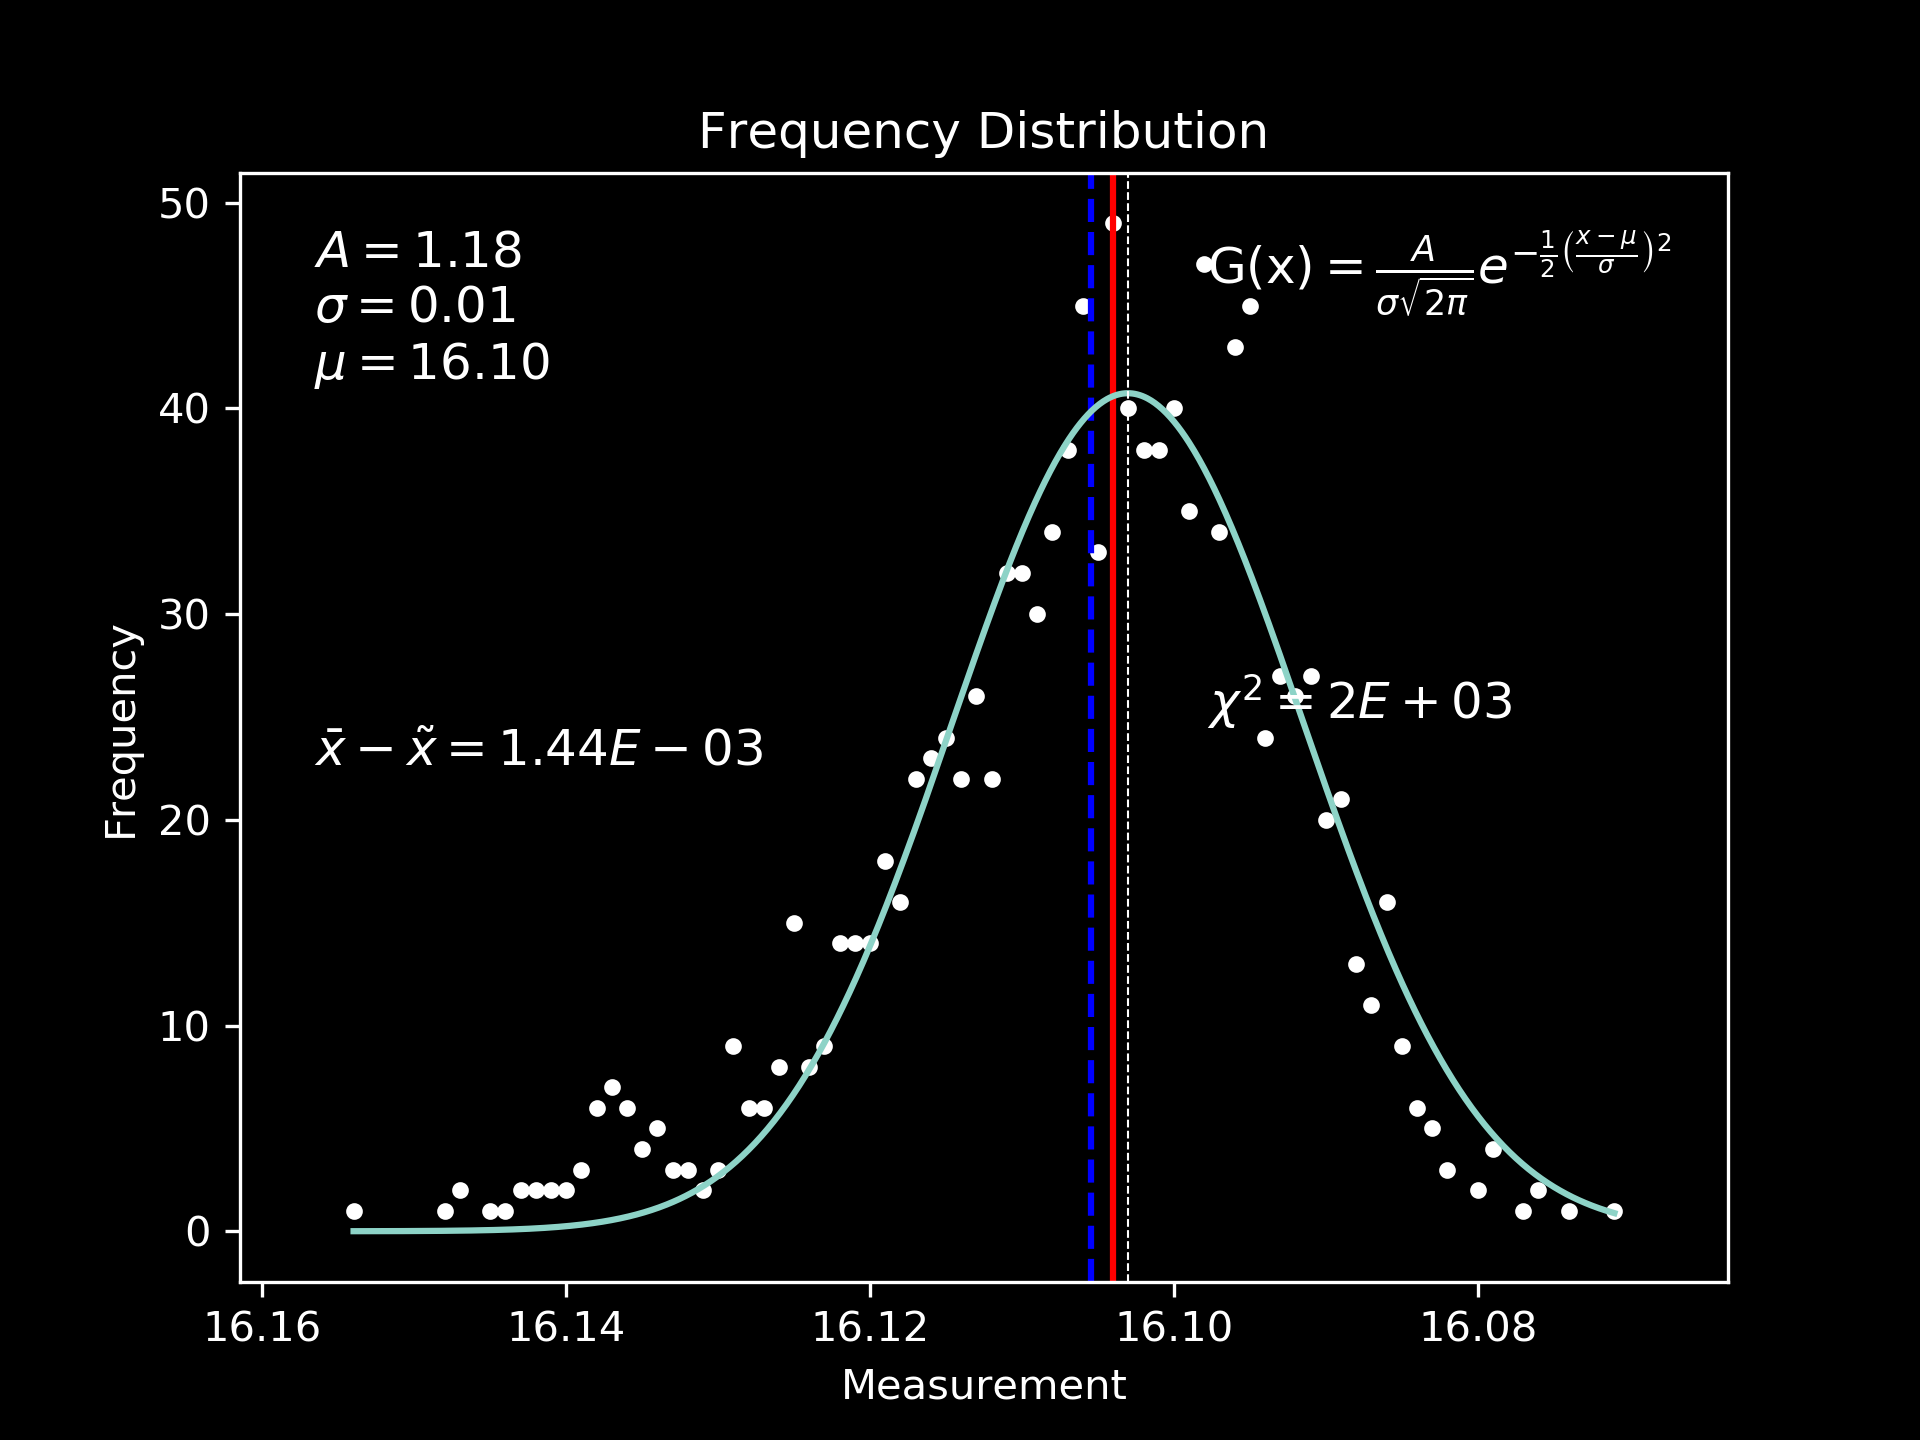
\includegraphics[width=\textwidth]{freq_dist}
\label{fig:freq_dist}
\end{figure}
\end{frame}

\begin{frame}
\[
\mathcal{R}
= \frac{x-\bar x}{\vqty{\Delta x}}
\qquad
\text{$x$ is the magnitude measuremnet}
\]

\[
\mathrm{PDF} \ f(x)
\arr \mathrm{CDF} \ F(x)
\]

\[
F(x) = P(X \leq x) = \frac{1}{n} \int _{\infty}^x f_X(t)\ \dd t
\]
\end{frame}


\begin{frame}
\begin{figure}[h]
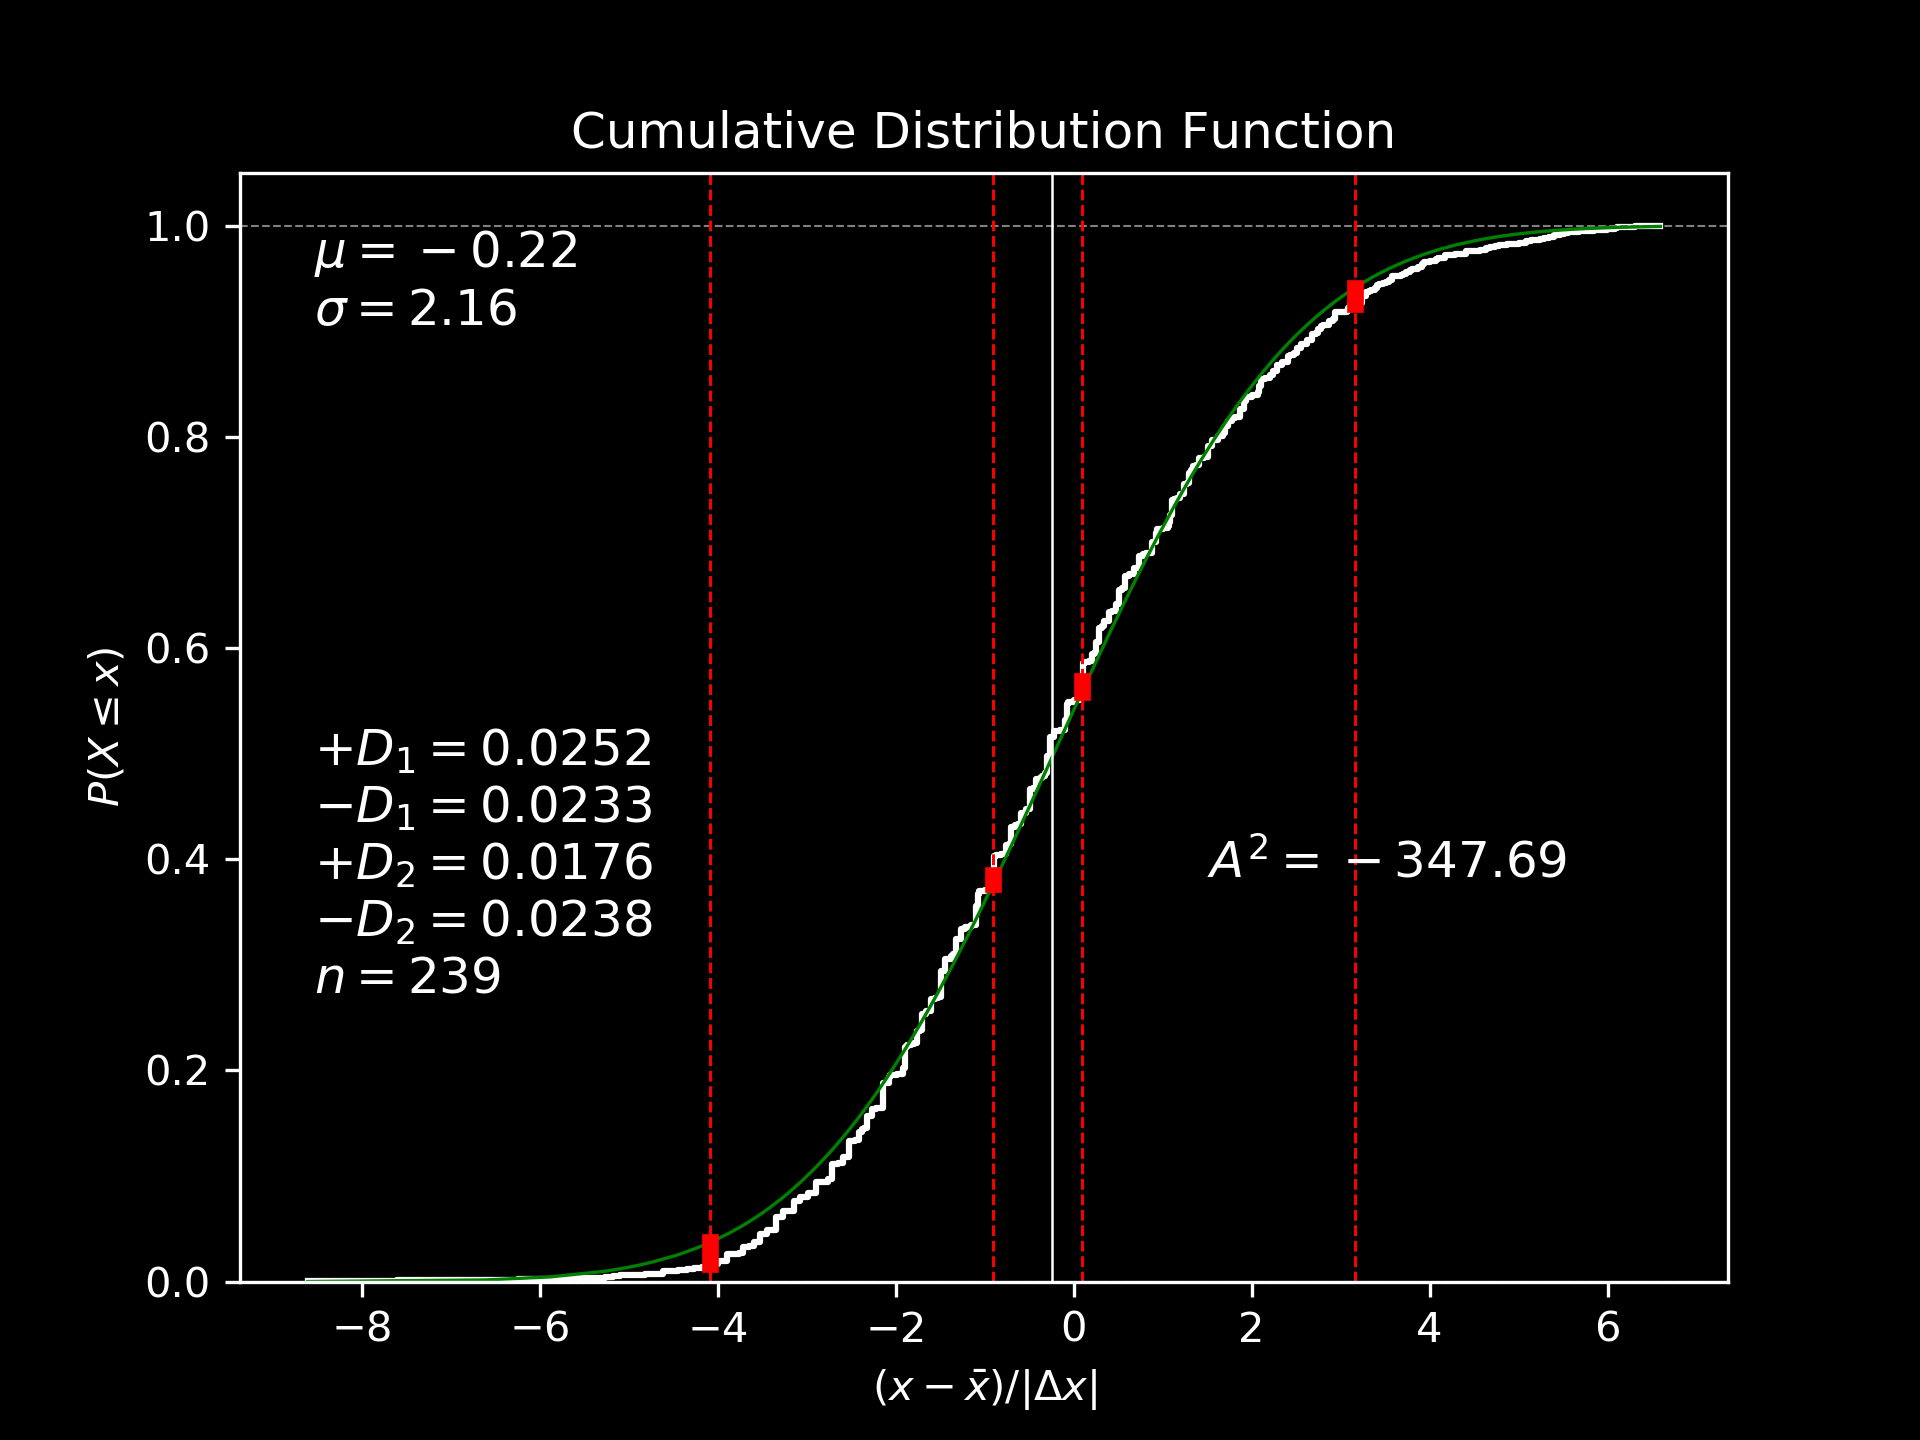
\includegraphics[width=\textwidth]{cumu_dist}
\centering
\label{fig:cumu_dist}
\end{figure}
\end{frame}


\begin{frame}
\frametitle{student's $t$-distribution}
\[
f(t; t_0, \nu) = \frac{1}{\sqrt{\nu}\ \mathrm{B}(\frac12, \frac{\nu}{2})}
\left( 1+\frac{(t-t_0)^2}{\nu}\right)^{-\frac{\nu+1}{2}}
\qquad
\mathrm{B}(x,y) = \int_0^1t^{x-1}(1-t)^{y-1}\ \dd t
\]
\begin{figure}[h]
\centering
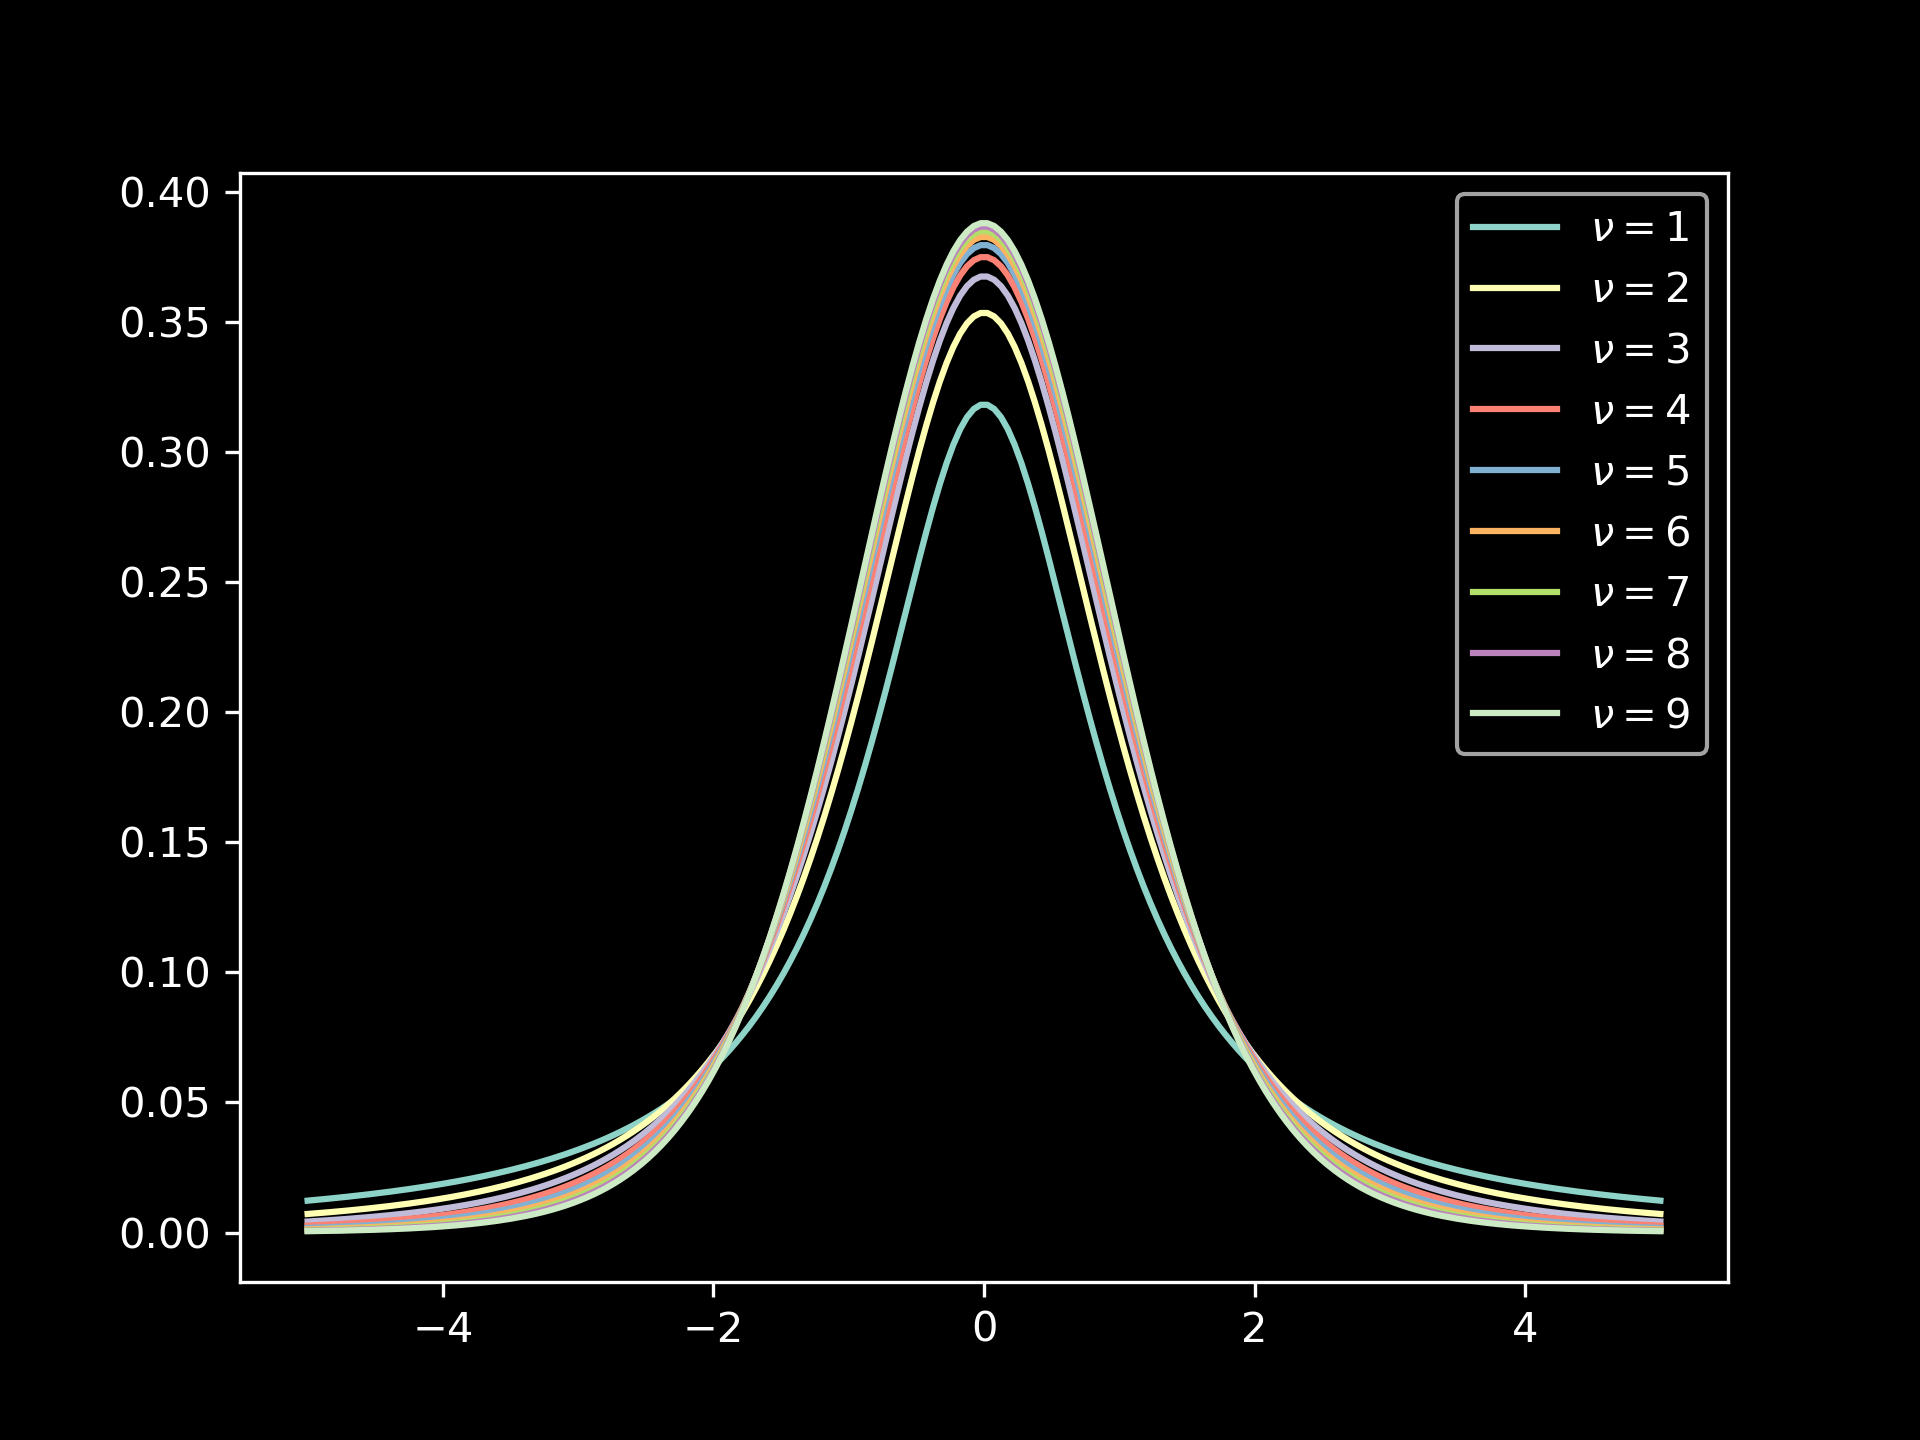
\includegraphics[width=6cm]{t_dist}
\label{fig:t_dist}
\end{figure}
\begin{equation*}
\begin{aligned}
F(t; u_0, \nu) &= \int_{-\infty}^tf(u)\ \dd u
\\&= \int_{-\infty}^t
\frac{1}{\sqrt{\nu}\ \mathrm{B}(\frac12, \frac{\nu}{2})}
\left( 1+\frac{(u-u_0)^2}{\nu}\right)^{-\frac{\nu+1}{2}}
\ \dd u
\end{aligned}
\end{equation*}
\end{frame}


\begin{frame}
\begin{figure}[h]
\centering
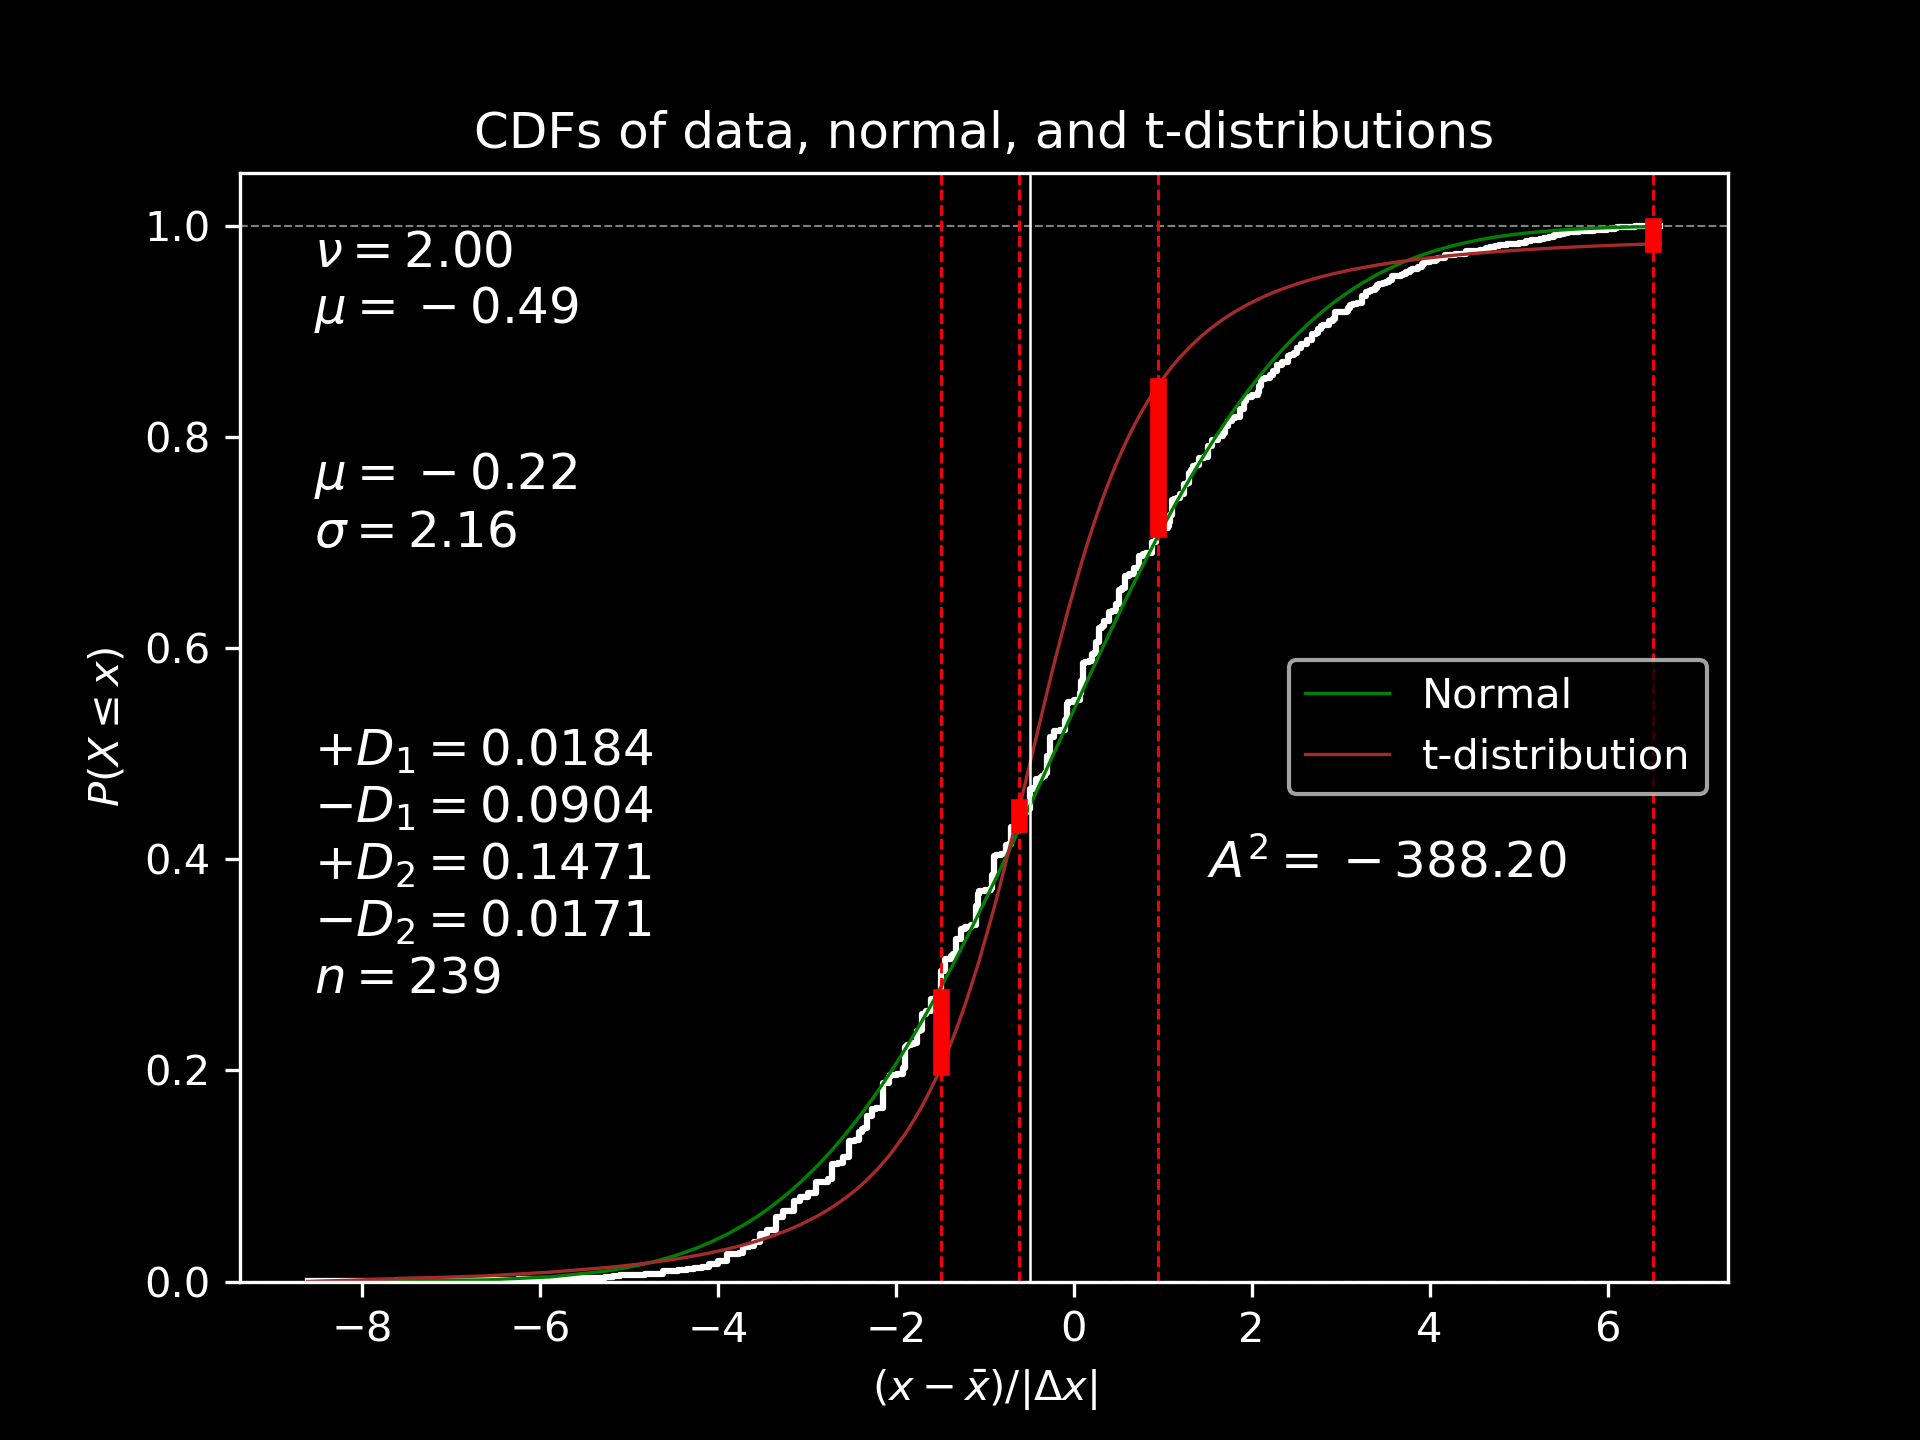
\includegraphics[width=\textwidth]{t_cdf}
\label{fig:t_cdf}
\end{figure}
\end{frame}


\begin{frame}
\frametitle{Cauchy / Lorentzian Distribution}
\[
f(x; x_0, \gamma)
=\frac{1}{\pi\gamma}\left[1+\pqty{\frac{x-x_0}{\gamma}}^2\right]
=\frac{1}{\pi\gamma}\left[\frac{\gamma ^2}{(x-x_0)^2+\gamma ^2}
\right]
\]
\begin{figure}[h]
\centering
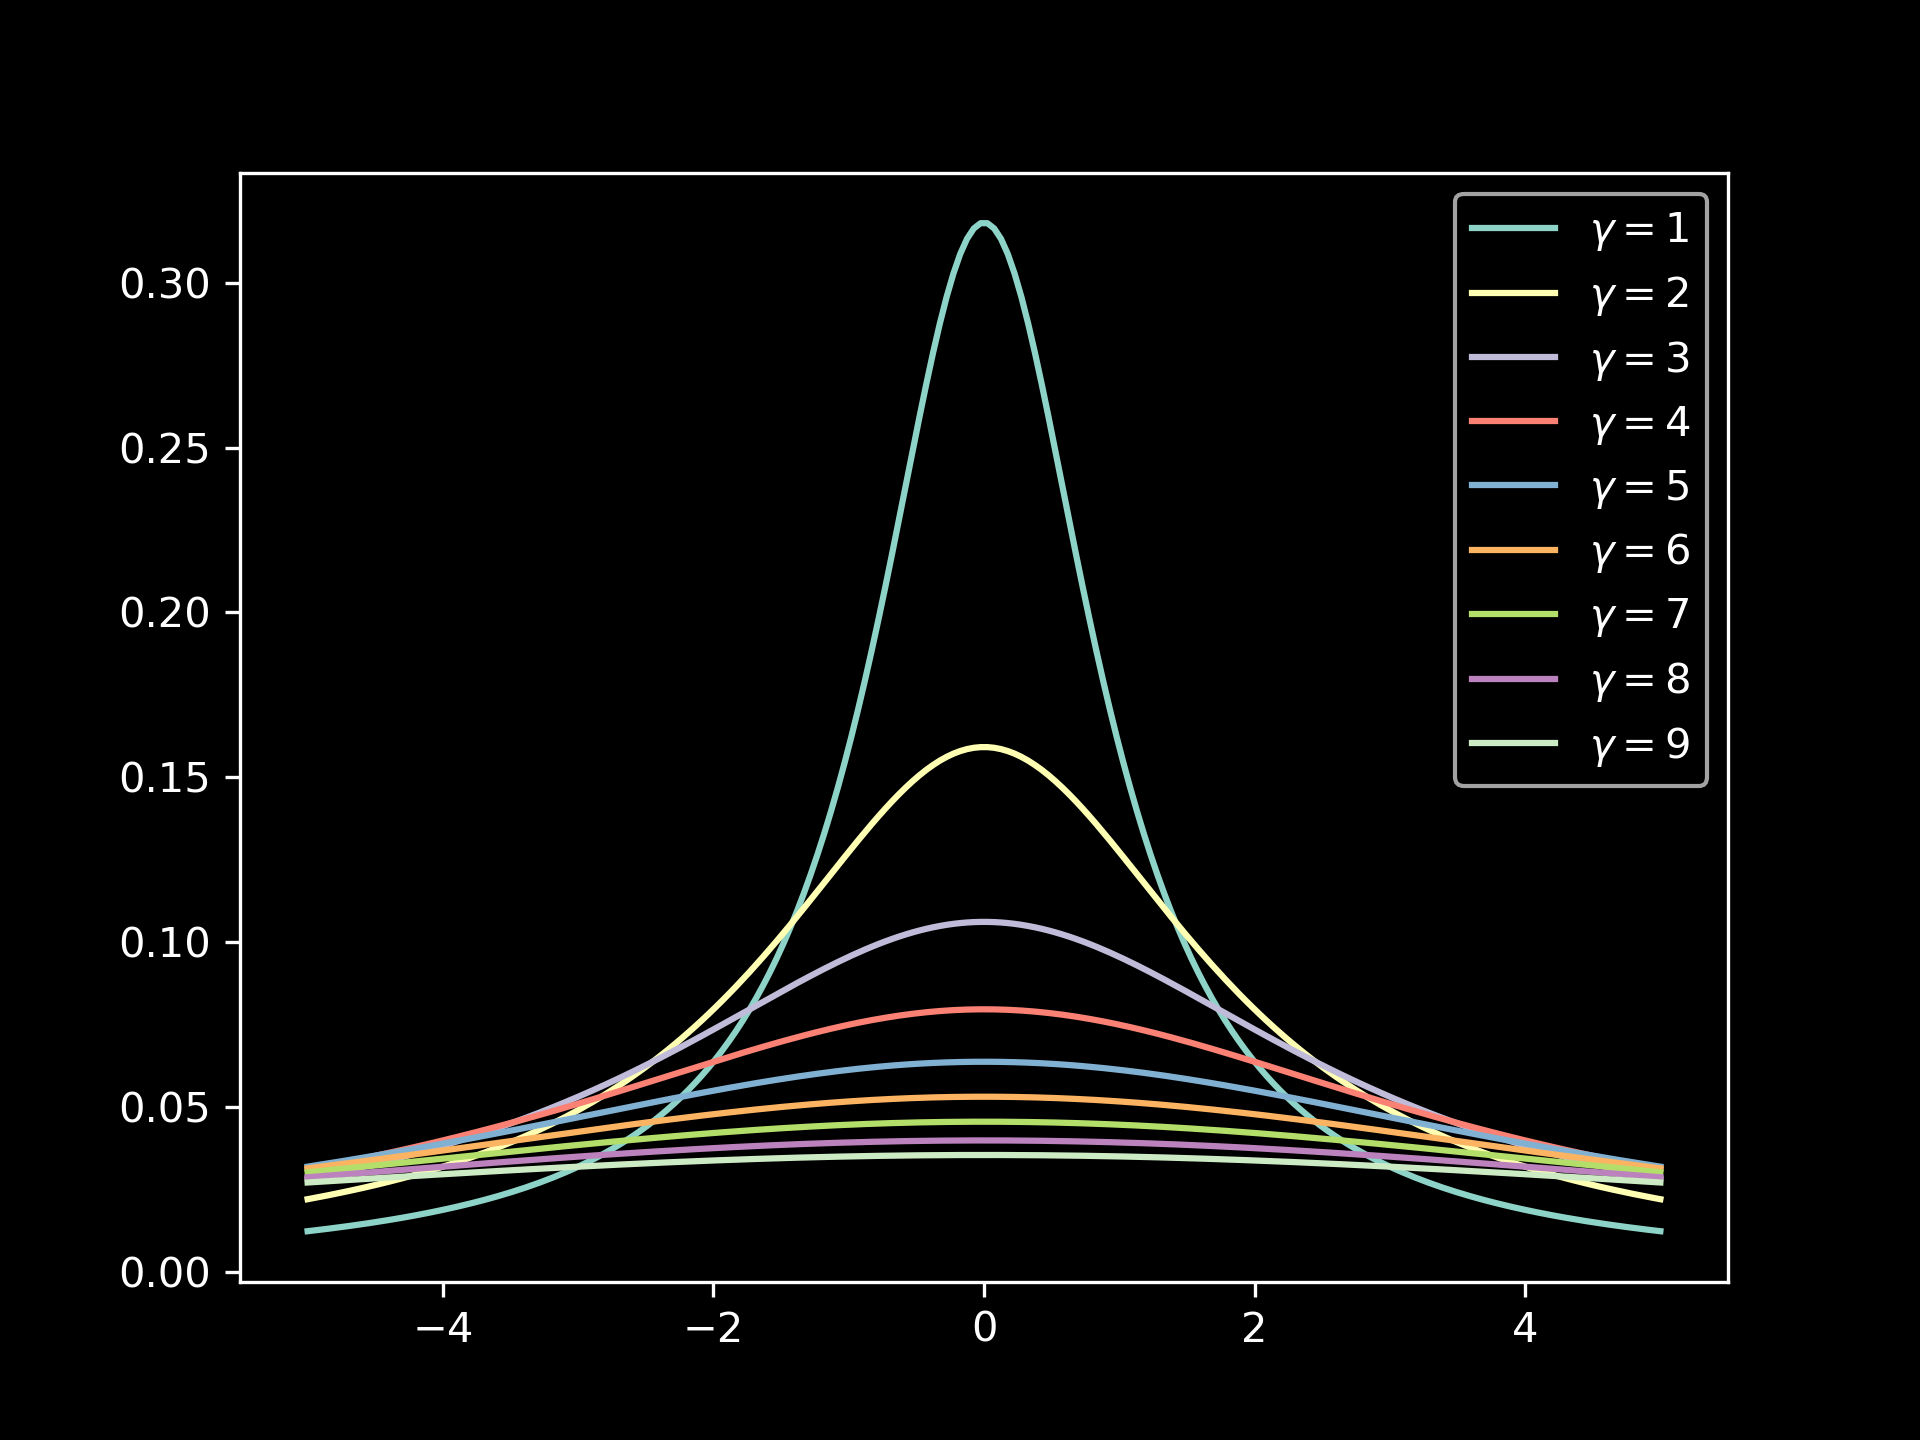
\includegraphics[width=6cm]{lo_dist}
\label{fig:lo_dist}
\end{figure}

\begin{equation*}
\begin{aligned}
F(x;x_0, \gamma) &=
\int _{-\infty}^x f(t)\ \dd t
\\&=\frac{1}{\pi}
\arctan\pqty{\frac{x-x_0}{\gamma}}+\frac12
\end{aligned}
\end{equation*}
\end{frame}



\begin{frame}


\begin{figure}[h]
\centering
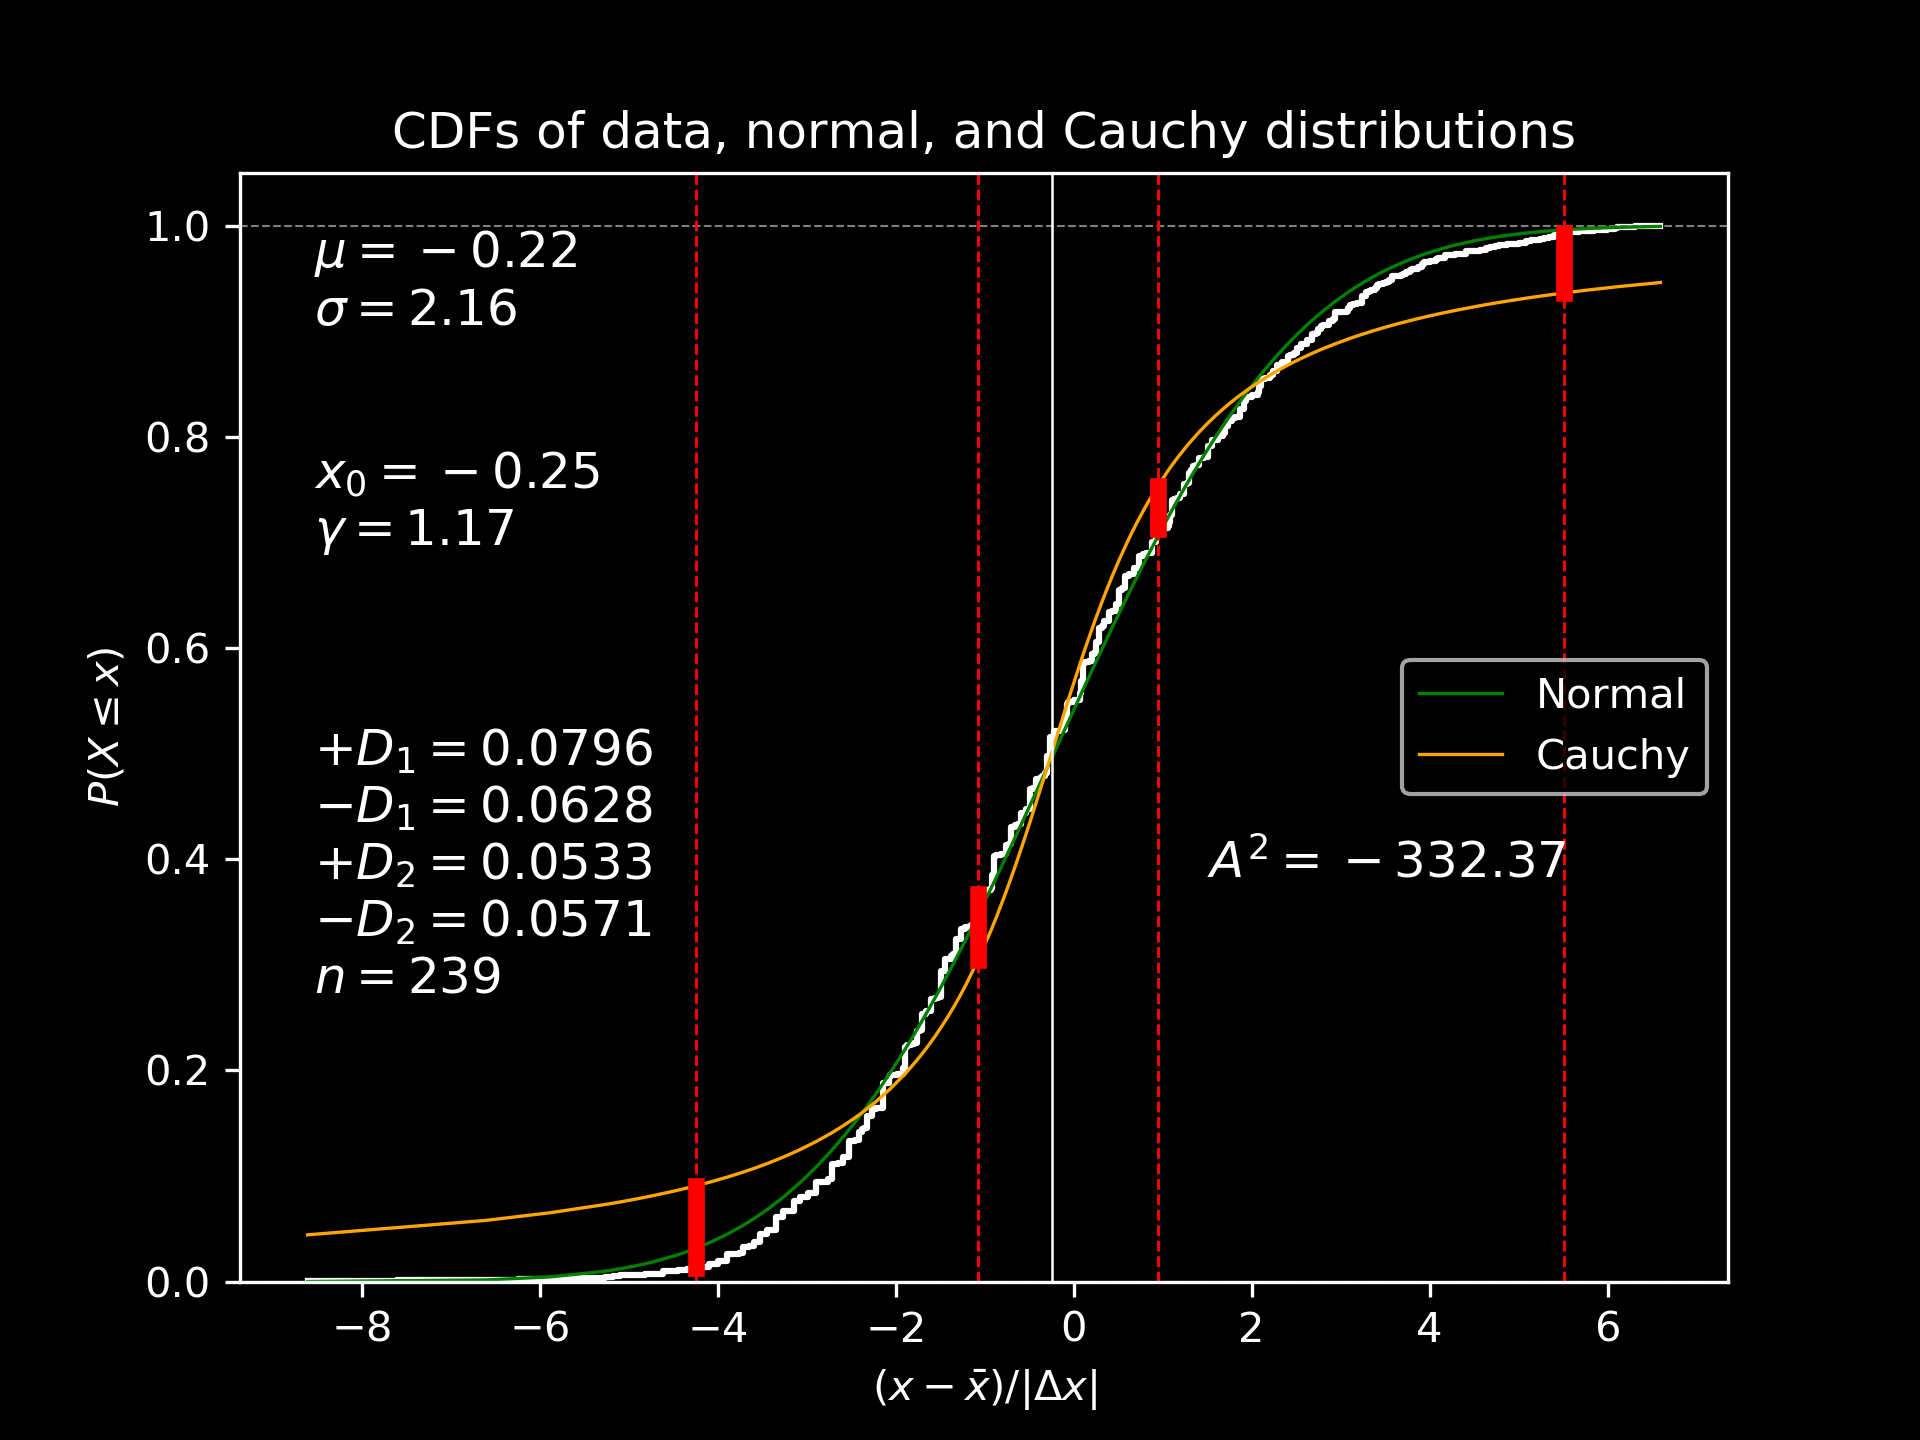
\includegraphics[width=\textwidth]{cauchy_cdf}
\label{fig:cauchy_cdf}
\end{figure}
\end{frame}


\begin{frame}
\frametitle{Error Correcting}

\[
\Delta x \rightarrow \sqrt{\Delta x^2 + C^2}
\qq{so that}
\mathcal{R} = \frac{x-\bar x}{\sqrt{\Delta x^2 + C^2}}
\]
\begin{figure}[h]
\centering
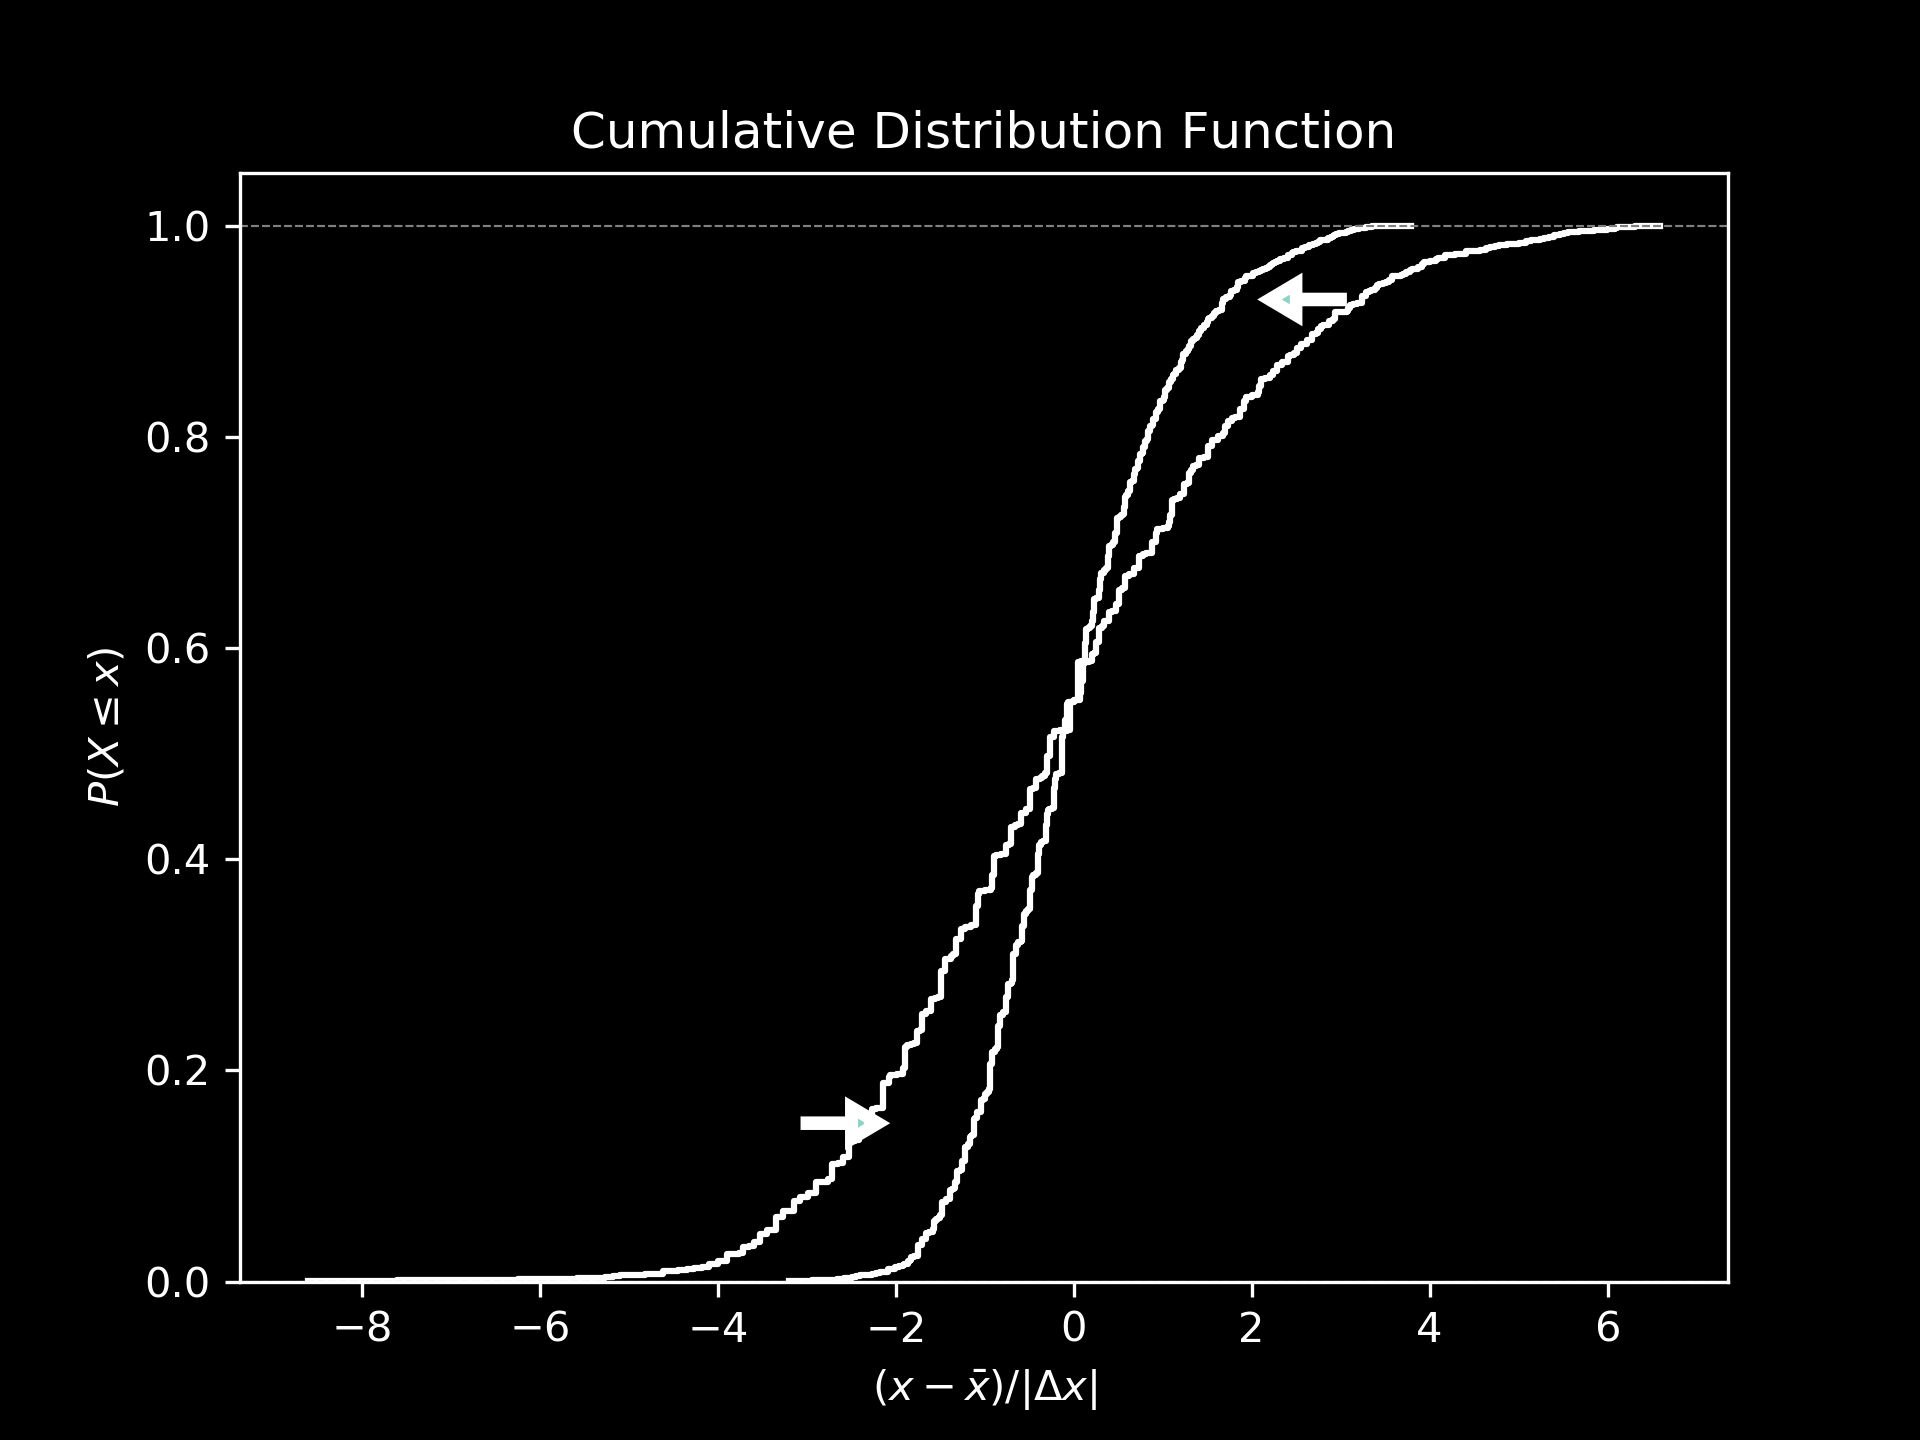
\includegraphics[width=10cm]{err_cor1}
\label{fig:err_cor1}
\end{figure}
\end{frame}


\begin{frame}
\[
\mathcal{S}(C, \mu, \sigma) = \sum_{i=1}^{n}
\bqty{F_\mathrm{G} (\mathcal{R}_i(C); \mu, \sigma)
  -F(\mathcal{R}_i(C))}^2
\cdot w(\mathcal{R}_i(C); \mu)
\]

\[
w(x;\mu, \alpha, \beta)
= \frac{\beta -1}{\alpha ^2}(x-\mu)^2 + 1
\]
\begin{figure}[h]
\centering
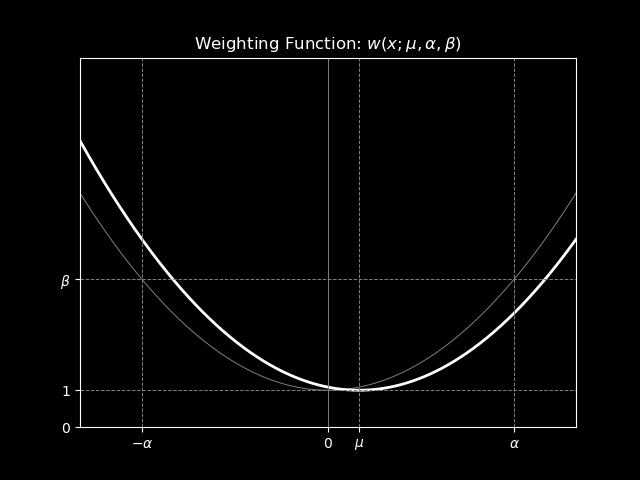
\includegraphics[width=10cm]{weight.png}
\end{figure}
\end{frame}

\begin{frame}
\begin{figure}[h]
\centering
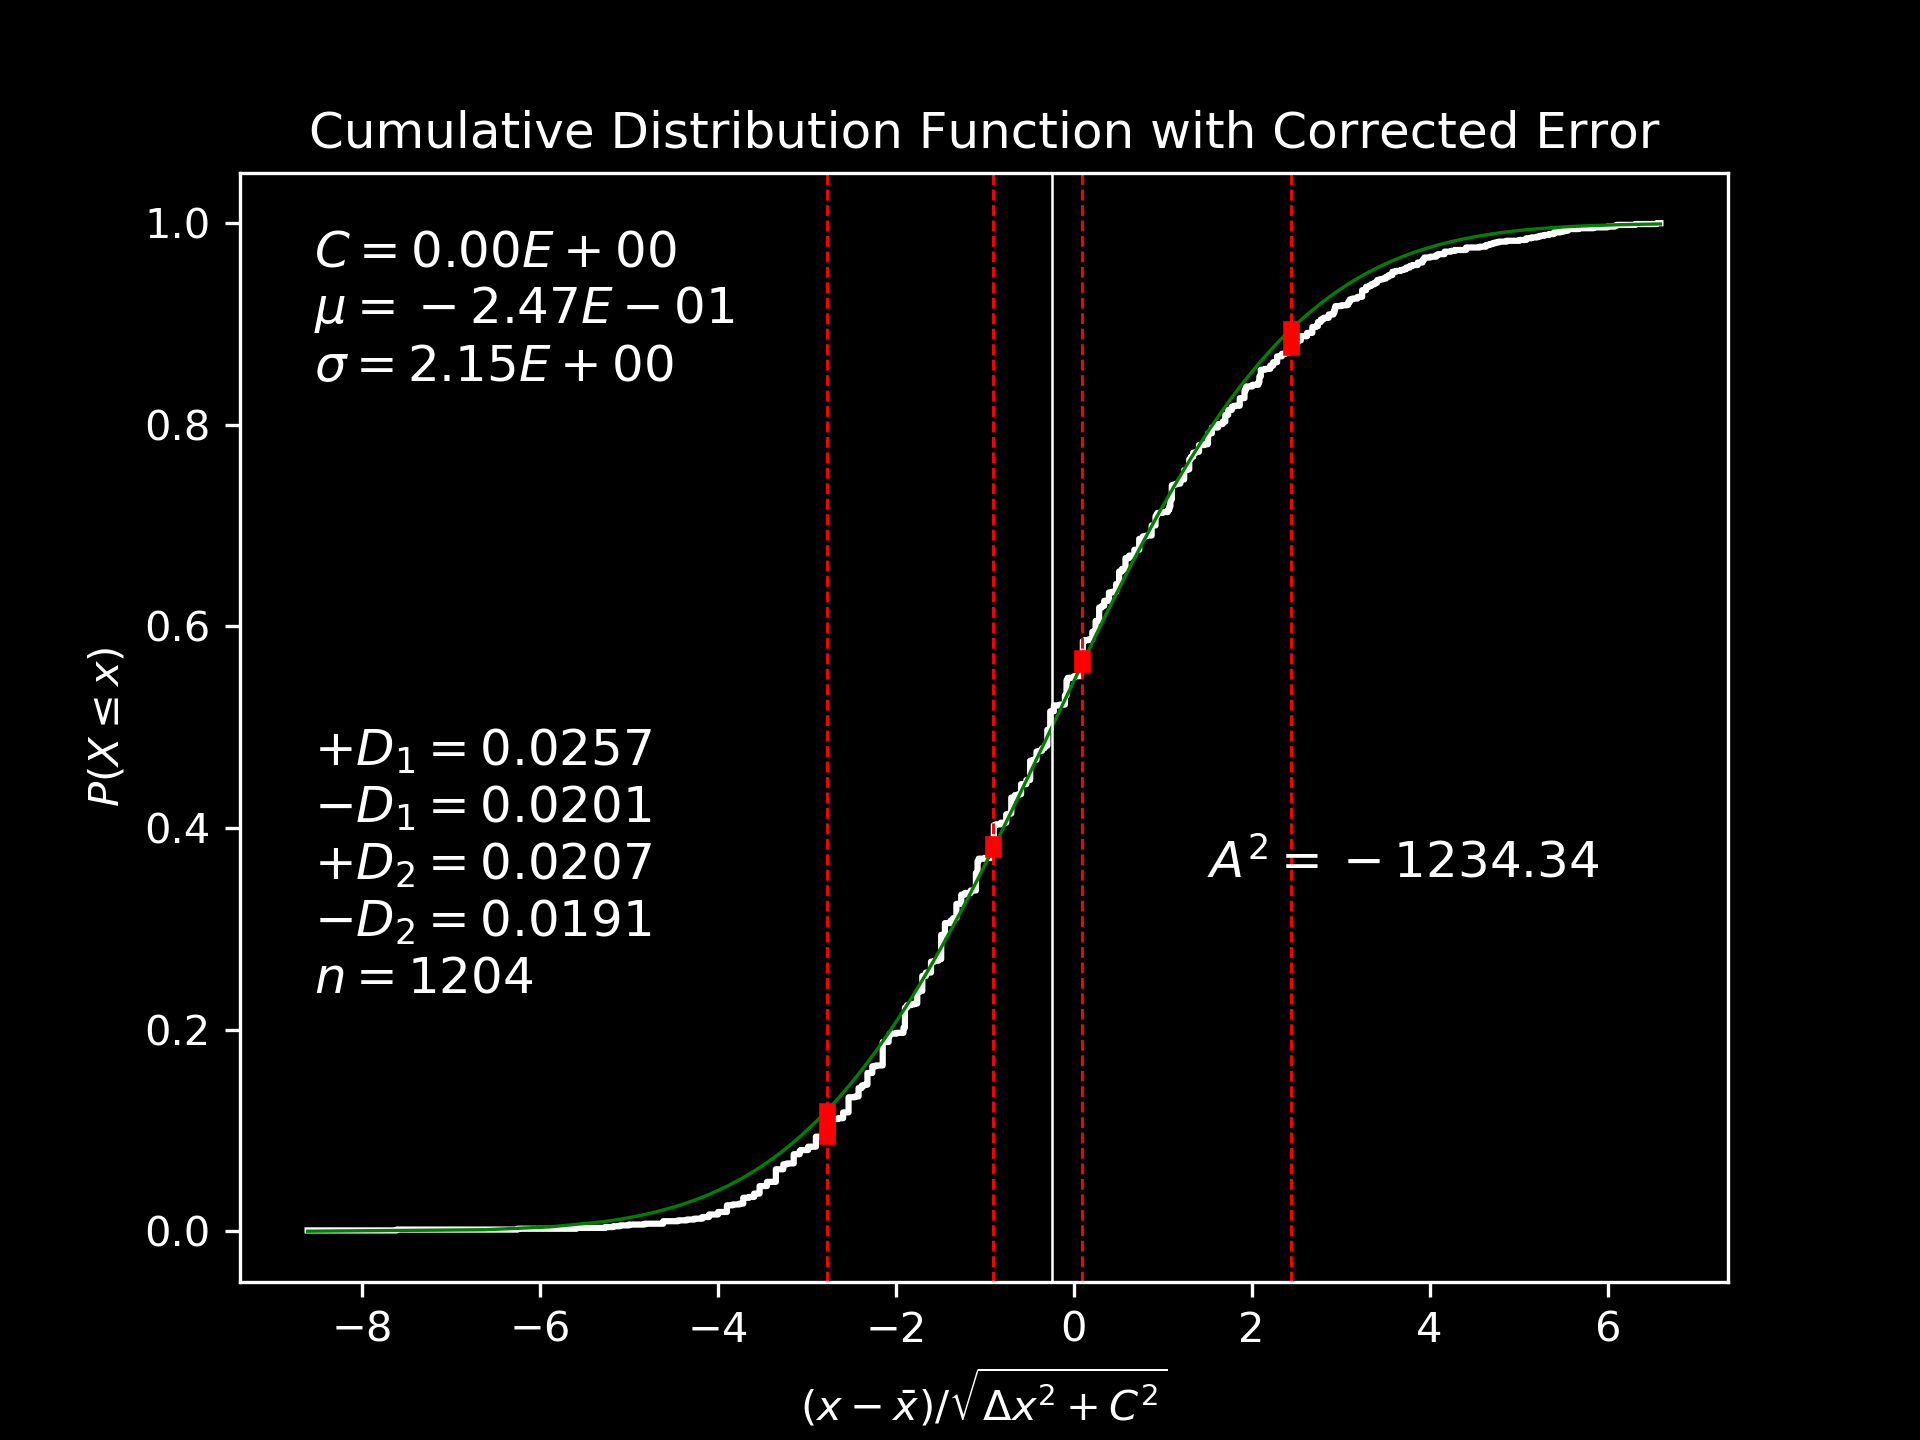
\includegraphics[width=\textwidth]{gauss_ec}
\label{ref:gauss_ec}
\end{figure}
\end{frame}

\begin{frame}
\begin{figure}[h]
\centering
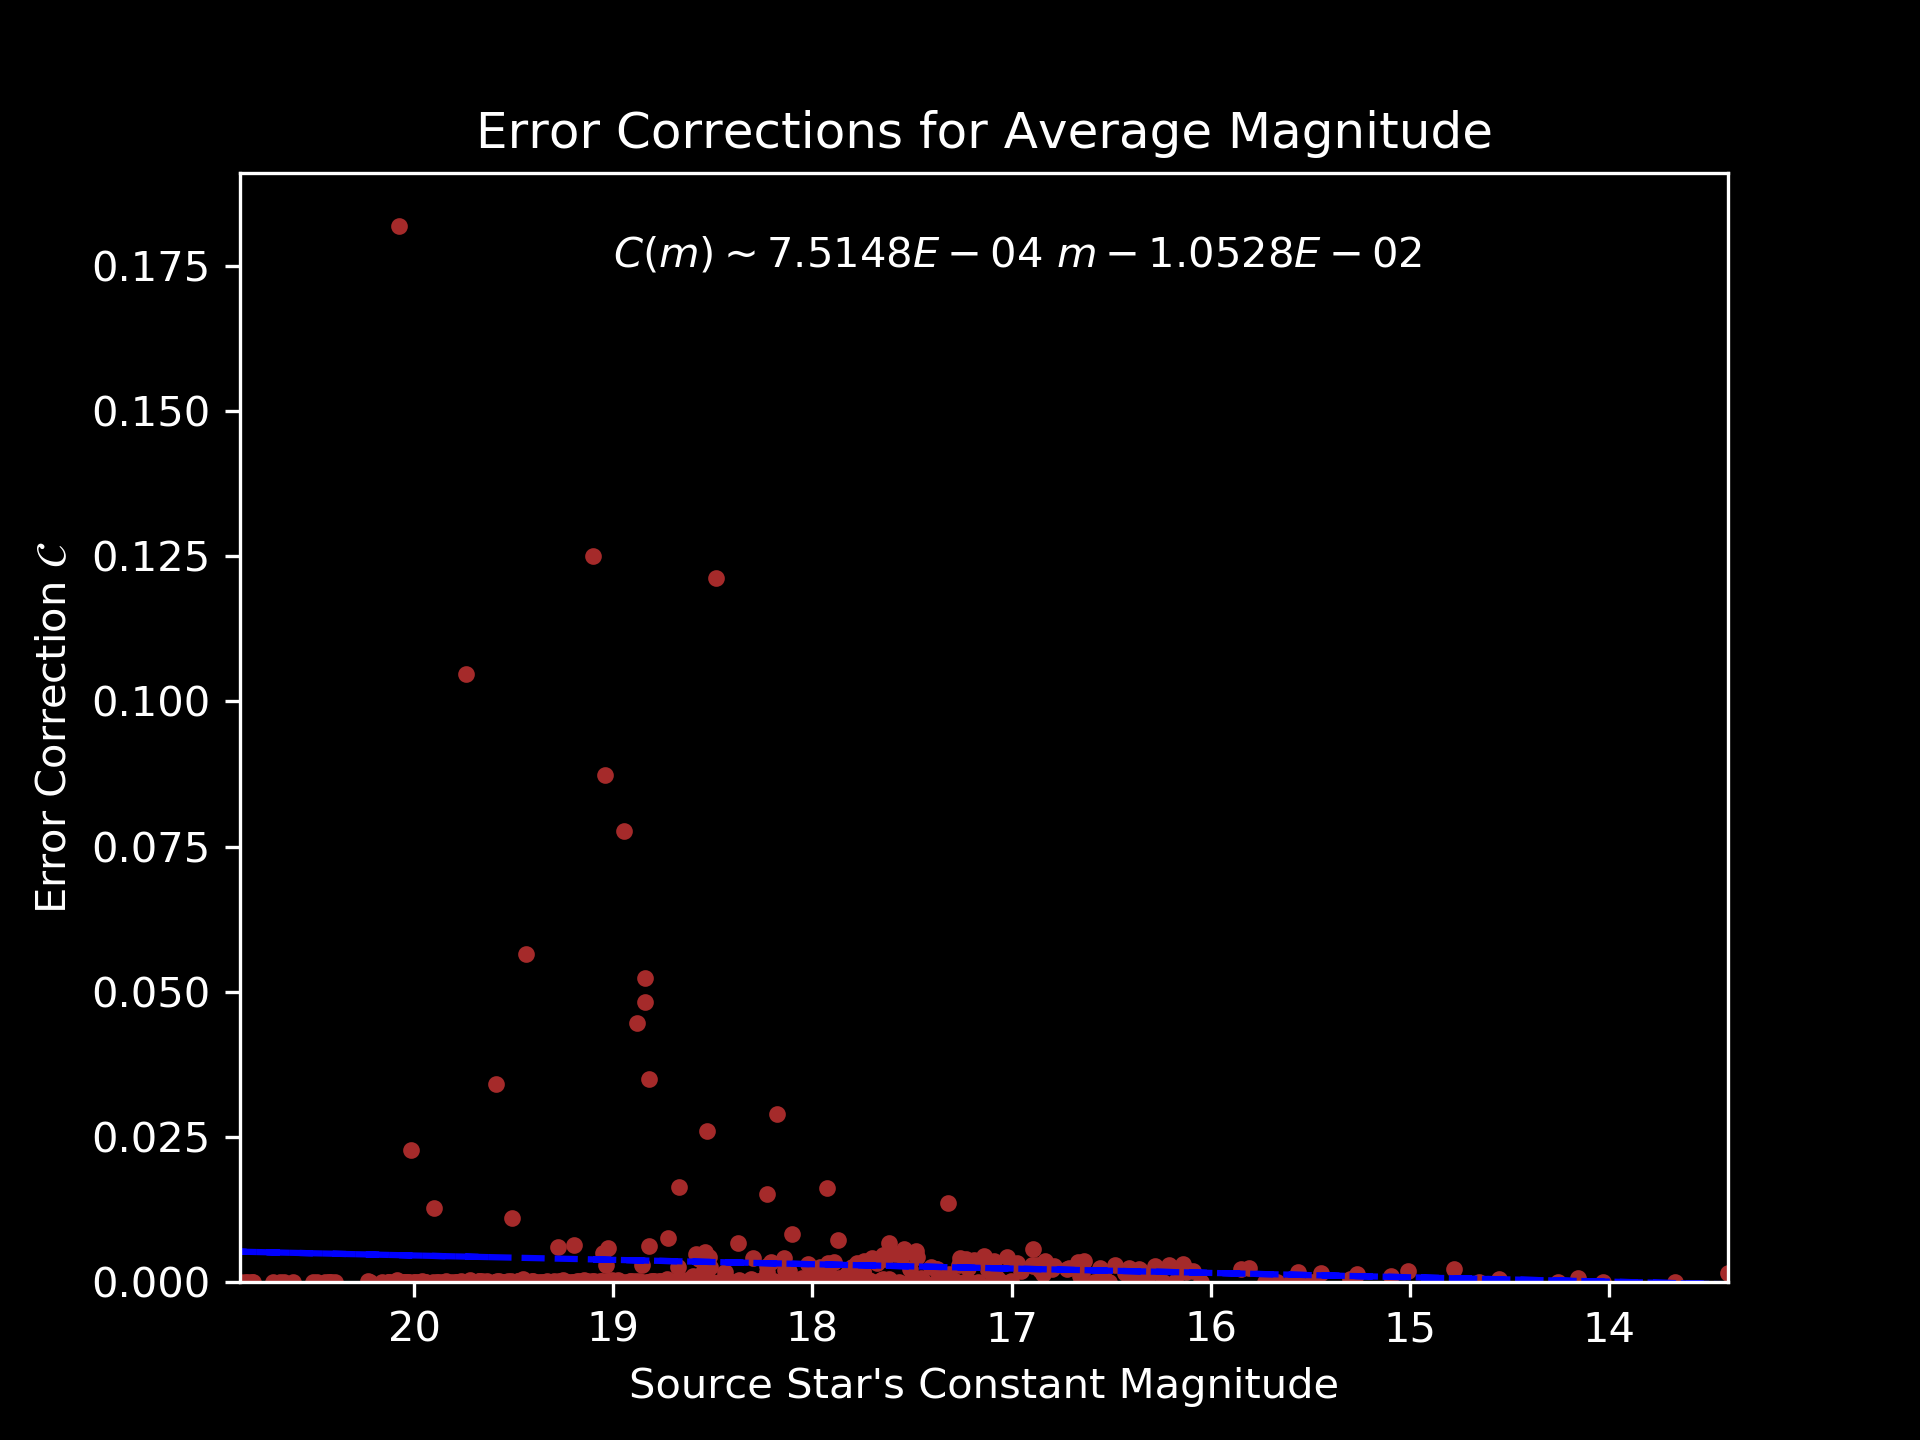
\includegraphics[width=\textwidth]{final}
\label{fig:final}
\end{figure}
\end{frame}



\end{document}
